\documentclass[conference]{IEEEtran}
\usepackage[T1]{fontenc}
\usepackage{microtype}
\usepackage{booktabs}
\usepackage{graphicx}
\usepackage{balance}
\usepackage{stfloats}
\usepackage[hidelinks]{hyperref}
\hypersetup{pdftitle={KVFold: Expanding Cache Capacity for LLM Agents with Lossless Compression},
            pdfsubject={ICDE demonstration paper}}
\title{KVFold: Expanding Cache Capacity for \mbox{LLM Agents} with Lossless Compression}
\author{\IEEEauthorblockN{Working draft}
\IEEEauthorblockA{Author information to be supplied}}
\raggedbottom
% Consistent space around floats; keep the IEEE text size and margins.
\setlength{\textfloatsep}{7pt plus 2pt minus 2pt}
\setlength{\dbltextfloatsep}{7pt plus 2pt minus 2pt}
\setlength{\intextsep}{7pt}
\begin{document}
\bstctlcite{kvfoldBibControl}
\maketitle

\begin{abstract}
Large language model (LLM) agents repeatedly reuse long prompt prefixes across
turns and resumed sessions, making key/value (KV) caching essential to avoid
redundant prefill computation. However, retaining these states in two-byte
bfloat16 (BF16) constrains serving at two levels: GPU memory bounds active
request concurrency, while external DRAM and NVMe capacity bounds how much
history survives before eviction forces recomputation. We present KVFold, a
lossless KV-cache compression system integrated with unmodified vLLM and
LMCache to turn saved bytes into usable capacity across GPU attention and
variable-length external storage. By preserving every BF16 low byte and
encoding frequent high bytes with calibrated short codes, KVFold expands
usable GPU KV capacity from 1.18M to 1.59M tokens on Qwen3-30B-A3B replays
under a 54~GB per-GPU budget. Attendees edit and restore a live prompt to
inspect prefix reuse and verify KV integrity after re-import, then compare
queueing and tiered history retention across recorded coding-agent runs.
\end{abstract}

\section{Introduction}
Key/value (KV) caching avoids repeated prefill computation by reusing attention
states across generation steps and shared-prefix requests. This reuse is
critical for LLM agents, whose multi-turn transcripts and subagent calls share
long contexts. Retaining these states, however, demands substantial capacity:
Qwen3-30B-A3B consumes 96~KB of bfloat16 (BF16) KV per token across all layers
(48~KB per rank at tensor-parallel degree~2). Consequently, capacity constrains
serving at two distinct levels---GPU KV memory bounds active concurrency,
whereas external DRAM and NVMe tiers govern how much history survives before
eviction forces costly recomputation.

Existing serving systems mitigate this overhead through sharing and offloading:
vLLM's PagedAttention~\cite{vllm} shares fixed-size blocks across requests,
while LMCache~\cite{lmcache} and Mooncake~\cite{mooncake} offload KV caches
across host DRAM and storage tiers. Yet every retained
BF16 value still occupies two bytes. While lossy quantization~\cite{kivi}
alters KV values and requires accuracy requalification, lossless compression
preserves exact values by exploiting recurring BF16 bit patterns; for example,
SplitZip~\cite{splitzip} codes frequent exponents for prefill-to-decode
transfer and reassembles original sign and fraction bits at the receiver.

Extending lossless compression from transfer to persistent prefix caches
introduces three systems constraints to convert saved bytes into effective
capacity. First, restoring to a contiguous buffer requires an extra scatter
pass into scattered GPU pages. Second, keeping GPU blocks compressed saves
memory only if attention decompresses them on the fly at native kernel speed.
Third, external tiers retain more history only when the allocator assigns exact
encoded lengths and keeps length readback off the load path.

Addressing these constraints, we present KVFold, a lossless KV-cache
compression system built on offline-calibrated per-head codebooks. Because BF16
low bytes carry near-full entropy (7.97 of 8 bits) while high bytes are
strongly skewed---the top seven values cover $\approx$94\% of occurrences in
Qwen3-30B-A3B (top 14 cover 99.81\%)---KVFold keeps low bytes verbatim and
codes high bytes with fixed-width two-level symbols across two modes:
\begin{itemize}
\item \emph{Pool mode} keeps completed blocks compressed inside shared-budget
GPU pages. Decode attention fuses register decompression with tensor-core
computation, and the worker exports the same records to LMCache unchanged.
\item \emph{Tier mode} retains unmodified native BF16 GPU pages and stock
attention kernels. LMCache stores exact-length compressed objects across DRAM
and NVMe and restores chunks directly into scattered GPU pages.
\end{itemize}

\section{KVFold Architecture}
\label{sec:design}
\subsection{Overview}
Figure~\ref{fig:architecture} illustrates KVFold across the GPU, PCIe, and
external cache tiers. Unmodified vLLM (v0.30) schedules requests and allocates
128-token logical blocks, while the LMCache server (v0.5.6) accesses engine
blocks over CUDA IPC and manages L1~DRAM and L2~NVMe lookup, LRU eviction,
write-through, and prefetch. In pool mode (Fig.~\ref{fig:architecture}a), an
out-of-tree attention plugin compresses closed blocks into the GPU pool and
exports immutable pool objects unchanged across PCIe. In tier mode
(Fig.~\ref{fig:architecture}b), vLLM runs stock FlashAttention-3
(FA3)~\cite{fa3neurips} on native BF16 pages while LMCache invokes KVFold's GPU
codec on saves and restores. Incompressible tier chunks cross PCIe as raw BF16.

\begin{figure*}[t]
\centering
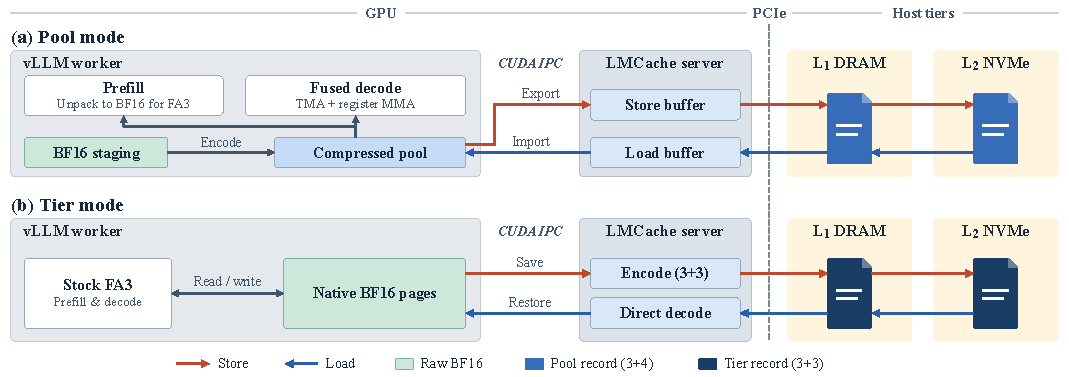
\includegraphics[width=0.96\textwidth]{images/KVFold_Fig1_Architecture.pdf}
\caption{KVFold integration across GPU memory, PCIe, and external cache tiers.
(a)~Pool mode stores compressed shared-budget pages on the GPU and exports them
unchanged to L1~DRAM and L2~NVMe. (b)~Tier mode retains native BF16 GPU pages
with stock FlashAttention-3 (FA3)~\cite{fa3neurips} and runs a server-side GPU
codec, transferring incompressible chunks as raw BF16.}
\label{fig:architecture}
\end{figure*}

\subsection{Lossless KV Encoding}
\label{sec:encoding}
Both modes store every BF16 low byte verbatim and encode the high byte (sign
plus upper seven exponent bits) using static offline-calibrated tables per
layer, KV head, and tensor (K or V). Inspired by lightweight database
compression---fixed-width codes with out-of-band exceptions~\cite{pfor,alp} and
lane-parallel layouts~\cite{fastlanes}---KVFold uses fixed-width symbols so
every warp lane reads at fixed offsets for lockstep parallel decoding. Each high byte first
receives a 3-bit primary code indexing the seven top entries in primary table
$P$, with \texttt{111} signaling an escape. The two modes specialize secondary
width and layout for their decoders: \emph{tier records} use a 3+3 code
(3-bit secondary indexing seven entries in extended table $E$, with
\texttt{111} escaping to an 8-bit raw byte) so all 14 entries fit in 16~B of
registers for branchless GPU \texttt{PRMT} lookup over token-ordered streams;
\emph{pool records} widen the secondary selector to 4~bits (3+4: 15 entries in
$E$, \texttt{1111} escaping to a 4~B raw patch), adding only 0.1\% to record
size while bounding per-warp raw patches so fused register decompression stays
loop-free.

Figure~\ref{fig:record}a traces pool-mode Direct, Extended, and Raw fallback
paths on \texttt{3C12}, \texttt{3956}, and \texttt{4178} (verified bit-exact
against a CPU reference). Offline calibration on a single 1,024-token agent
pass produces 8.4~KB of tables for Qwen3-30B-A3B; across seven prompt domains
on Qwen3-30B-A3B and GLM-4-9B-Chat-1M, mean tier sizes stay within
70.6\%--70.9\% of raw BF16 ($<$0.1 percentage point gain from domain-specific
recalibration).

\begin{figure}[!ht]
\centering
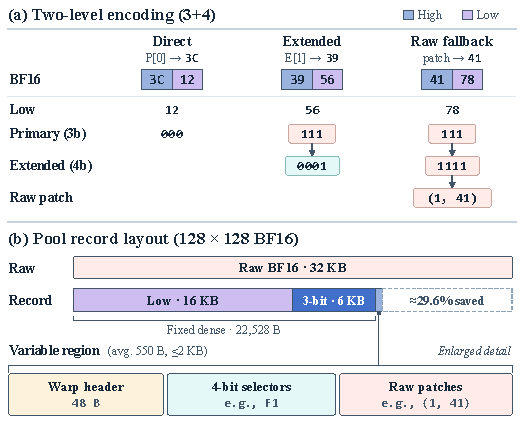
\includegraphics[width=0.97\columnwidth]{images/KVFold_Fig2_Encoding.pdf}
\caption{(a)~Two-level BF16 high-byte encoding in pool mode (3+4), where $P$
and $E$ are calibrated primary and extended tables (tier mode uses 3+3 for
register \texttt{PRMT} lookup). (b)~A 128-token pool record versus 32~KB of raw BF16. The variable region is drawn
at its mean size (550~B, capped at 2~KB) and enlarged below.}
\label{fig:record}
\end{figure}

\subsection{Pool Mode: GPU-Resident KV}
\label{sec:pool}
KVFold stages each active request's growing block in raw BF16 and encodes it
immediately after token~128 completes. Each pool record
compresses one 128$\times$128 BF16 tensor (32~KB raw; one block, layer, head,
and K/V) permuted into tensor-core MMA fragment order: a fixed 22,528~B dense
part (16~KB low bytes + 6~KB 3-bit codes) plus a $\le$2~KB variable region
(48~B warp header, 4-bit selectors, 4~B raw patches; avg.\ 550~B;
Fig.~\ref{fig:record}b). All $2H$ K/V records of a block and layer share one
compressed page with a pooled variable budget; at $H{=}4$, pages shrink from
256~KB to 186~KB (1.38$\times$ raw blocks before deducting staging, overflow,
record-map, and prefill buffers). Parallel encoders claim page space via an
atomic fill counter and publish \emph{(address, length)} in a per-layer record
map; the rare records exceeding 2~KB or remaining page space (0.03\% in
serving) fall back to 32~KB raw overflow slots.

During \emph{prefill}, the plugin decodes cached pages into a BF16 workspace
for unmodified FA3 ($\le$3\% overhead). During \emph{decode}, a fused kernel
uses the Tensor Memory Accelerator (TMA) to prefetch records one step ahead
into dual shared-memory slots, decompresses each thread's 64 scalars directly
into registers without writing KV back to global memory, and executes
tensor-core MMAs with online softmax before merging partial states across page
ranges. Fixed padded-batch launch metadata preserves decode-only CUDA graph
replay; every KV bit is exact, while accumulation order matches FA3 up to
floating-point rounding. Completed blocks export behind a 4~KB-aligned header
for unchanged storage in LMCache and re-import directly into GPU pages via
atomic fill counters (falling back to vLLM recomputation if validation fails).

\subsection{Tier Mode: External KV Storage}
\label{sec:tier}
Tier mode leaves vLLM's native BF16 pages and stock FA3 unchanged while
compressing chunks in LMCache. Each tier record bundles 128 tokens across all
layers per TP rank behind a 4~KB-aligned header with 4~KB tail padding for
\texttt{O\_DIRECT} NVMe I/O (falling back to raw if incompressible), splitting
each tensor into four streams (low, primary, secondary, raw) partitioned into
256-scalar tiles with an 8-tile grouped index (0.14 bits/scalar).

On stores, three GPU kernels compress directly from paged blocks without a
gather pass, while a background store worker waits on a CUDA event for batched
\emph{deferred length readback}, exact-length L1~DRAM allocation, and L2~NVMe
write-through so length readback never stalls loads. On loads, two CUDA streams
rotate four GPU load buffers to overlap PCIe DMA with multi-process GPU
decompression: each warp runs branchless \texttt{PRMT} lookup to restore tiles
straight into scattered GPU pages (using a scratch buffer only for raw or
partially shared leading chunks). On one H800 SXM (256 chunks, 3~GB of
Qwen3-30B-A3B KV), SplitZip decoded at 1,215~GB/s contiguously but dropped to
671~GB/s with page scatter (76.8\% stored), whereas KVFold restored directly
into scattered pages at 1,182~GB/s (70.9\% stored). End-to-end greedy decoding
matched raw tiers bit for bit on both Qwen3-30B-A3B and GLM-4-9B.

% Declare Fig. 3 near the end of Section II so IEEEtran places it at the top of Page 3.
\begin{figure*}[!t]
\centering
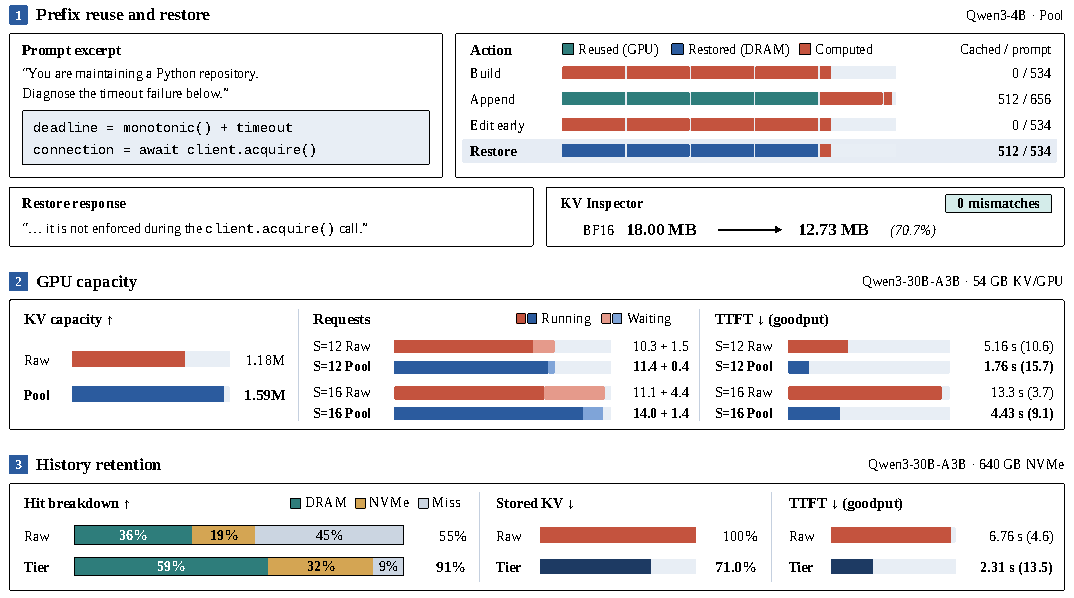
\includegraphics[width=0.94\textwidth]{images/fig3_console_update6.pdf}
\caption{Composite of selected views from the KVFold Console.
(1)~Live Qwen3-4B pool-mode interaction illustrating reused, restored, and
computed 128-token prefix blocks alongside the KV Inspector (18.00~MB BF16 to
12.73~MB encoded, zero export/import mismatches). (2)~Recorded AgentX GPU-capacity view
($P{=}64$, 54~GB KV/GPU, 400~GB DRAM, 2~TB NVMe): usable token capacity,
running vs.\ waiting requests in vLLM, and mean engine TTFT (with goodput in
req/min) at $S{=}12$ and $S{=}16$. (3)~Recorded AgentX history-retention view
($P{=}64$, $S{=}8$, 400~GB DRAM, 640~GB NVMe): prompt-token hit breakdown across
DRAM, NVMe, and misses, normalized stored KV size, and mean engine TTFT (with
goodput in req/min).}
\label{fig:views}
\end{figure*}

% Keep natural paragraph spacing below the full-width console figure.
\raggedbottom
\section{Demonstration Plan}
\label{sec:demo}
The eight-minute walkthrough in the KVFold Console (Fig.~\ref{fig:views})
begins with a live view of one coding-agent prompt across four requests.
After examining how the engine reuses and restores its prefix, attendees
explore two recorded views showing how GPU capacity affects request queues
and how external cache capacity affects history retention. Panel~1 runs live on
Qwen3-4B (pool mode, one H800 PCIe GPU, BF16 weights and KV); panels~2 and~3
show recorded InferenceX AgentX Claude Code runs~\cite{agentx} on Qwen3-30B-A3B
(FP8 weights, BF16 KV, two H800 SXM GPUs, TP~2), where $P$ counts live root
sessions and a FIFO proxy caps admitted requests at $S$. Engine TTFT excludes
proxy wait, and goodput counts requests/min with engine TTFT $\le 2$~s and mean
inter-token latency $\le 40$~ms.

\subsection*{Live Prefix Reuse and Restoration}
Attendees drive four interactive prompt actions on a Python repository
debugging task. Clicking \emph{Build} computes all 534 prompt tokens and
asynchronously exports completed 128-token compressed blocks to LMCache DRAM.
Clicking \emph{Append} adds a test instruction. The engine reuses 512 cached
tokens (teal in Fig.~\ref{fig:views}, panel~1), recomputes the original prompt's
22-token tail, and computes 122 new tokens. Next, \emph{Edit early} changes ``Python'' to
``TypeScript'' inside the first 128-token block, invalidating prefix reuse so
all 534 tokens recompute. Clicking \emph{Restore} waits for pending external saves, flushes the GPU prefix
cache, and replays the original prompt, restoring 512 tokens directly from
LMCache DRAM into the compressed GPU pool (blue blocks) and returning the
identical diagnosis.

After \emph{Build}, the \emph{KV Inspector} exports one 128-token block
(36 layers, 576 records) through host memory and re-imports it into a separate
GPU scratch store. It reports the footprint (18.00~MB BF16 $\rightarrow$
12.73~MB encoded, 70.7\%). The BF16 bytes decoded before export and after
import have matching SHA-256 digests and zero byte mismatches across all layers.

% Declare the paired tables on Page 3 so IEEEtran places them cleanly at the top of Page 4.
\begin{table*}[!t]
\begin{minipage}[b]{\columnwidth}
\centering
\caption{GPU capacity (54~GB KV/GPU, $P{=}64$, 400~GB DRAM, 2~TB NVMe,
0.94 hit share); Waiting and TTFT are means.}
\label{tab:gpu}
\small
\setlength{\tabcolsep}{3pt}
\begin{tabular*}{\columnwidth}{@{\extracolsep{\fill}}rlrrrr@{}}
\toprule
$S$ & Mode & KV tokens & Waiting &
\begin{tabular}[t]{@{}r@{}}TTFT\\(s)\end{tabular} &
\begin{tabular}[t]{@{}r@{}}Goodput\\(req/min)\end{tabular} \\
\midrule
12 & Raw  & 1.18M & 1.5 & 5.16 & 10.6 \\
12 & Pool & 1.59M & 0.4 & 1.76 & \textbf{15.7} \\
16 & Raw  & 1.18M & 4.4 & 13.3 & 3.7 \\
16 & Pool & 1.59M & 1.4 & 4.43 & \textbf{9.1} \\
\bottomrule
\end{tabular*}
\end{minipage}\hfill
\begin{minipage}[b]{\columnwidth}
\centering
\caption{History retention ($P{=}64$, $S{=}8$, 400~GB DRAM). Cached combines
DRAM and NVMe/GPU hit shares; TTFT is mean engine TTFT.}
\label{tab:tiers}
\small
\setlength{\tabcolsep}{3pt}
\begin{tabular*}{\columnwidth}{@{\extracolsep{\fill}}llrrr@{}}
\toprule
NVMe & Mode & Cached &
\begin{tabular}[t]{@{}r@{}}TTFT\\(s)\end{tabular} &
\begin{tabular}[t]{@{}r@{}}Goodput\\(req/min)\end{tabular} \\
\midrule
640~GB & Raw  & 0.55 & 6.76 & 4.6 \\
640~GB & Tier & 0.91 & 2.31 & \textbf{13.5} \\
2~TB   & Raw  & 0.94 & 1.69 & 15.1 \\
2~TB   & Tier & 0.94 & 1.73 & 15.1 \\
\bottomrule
\end{tabular*}
\end{minipage}
\end{table*}

\subsection*{GPU Capacity under Concurrent Load}
The recorded views show how live serving metrics guide mode selection. When
external tiers already retain the active working set (0.94 cached-token share
at 400~GB DRAM and 2~TB NVMe), rising concurrency makes GPU KV capacity the
primary bottleneck. Under a 54~GB per-GPU KV budget, pool mode holds 1.59M
usable tokens (1.34$\times$ raw's 1.18M) after reserving 1.3~GB inside the
budget for staging, overflow, record maps, and prefill workspace; cache-server
CUDA contexts and transfer buffers lie outside this budget.

At $S{=}8$, neither pool experiences appreciable queueing (raw and pool goodput
reach 15.1 and 16.3~req/min). Attendees toggle $S{=}12$ and $S{=}16$ in the
console (Fig.~\ref{fig:views}, panel~2; Table~\ref{tab:gpu}) to watch the raw
pool saturate: at $S{=}12$, raw builds a mean waiting queue of 1.5 requests and
triples mean engine TTFT to 5.16~s, whereas pool mode keeps queueing flat
(0.4 waiting), cuts mean engine TTFT to 1.76~s, and lifts goodput from 10.6 to
15.7~req/min---matching raw's uncongested $S{=}8$ performance while admitting
50\% more concurrent requests. At $S{=}16$, pool mode sustains 14.0 running
requests (vs.\ 11.1 raw) and achieves 2.5$\times$ higher goodput (9.1 vs.\
3.7~req/min).

\subsection*{History Retention under Storage Pressure}
When high miss rates or heavy NVMe traffic indicate external tier exhaustion,
attendees switch to the history-retention view (Fig.~\ref{fig:views}, panel~3;
Table~\ref{tab:tiers})
and compare 640~GB against 2~TB NVMe at $S{=}8$. Both arms use unmodified
native GPU pages, stock FA3, and identical LMCache LRU, write-through, and
prefetch policies; tier mode's store and rotating load buffers occupy
approximately 2.5~GB per GPU outside the KV budget.

At 640~GB NVMe, raw LMCache falls off its LRU eviction cliff: cached-token
share collapses to 0.55 (36\% DRAM, 19\% NVMe, 45\% recomputed misses), pushing
mean engine TTFT to 6.76~s and goodput down to 4.6~req/min. Compressing stored
KV to 71.0\% of raw bytes makes the tiers behave like 1.4$\times$ larger raw
tiers---lifting total cached share to 0.91 while promoting hits from NVMe into
DRAM (59\% DRAM, 32\% NVMe, 9\% misses). Tier mode thus cuts mean engine TTFT
by 2.9$\times$ (2.31~s) and raises goodput by 2.9$\times$ (13.5~req/min). At
2~TB NVMe, where raw capacity already holds the working set (0.94 hit share),
compression adds minimal overhead: goodput matches raw (15.1~req/min), mean
engine TTFT stays within 0.04~s (1.73 vs.\ 1.69~s), and prompt throughput drops
by only 2.2\% (26.9 vs.\ 27.5 thousand tokens/s).

\balance
\section*{Acknowledgment}
% Replace the reserved space below with two or three lines of acknowledgments.
\par\vspace*{3\baselineskip}

\bibliographystyle{IEEEtran}
\bibliography{references}
\end{document}
